\documentclass[../dissertation.tex]{subfiles}

\begin{document}
%%%%% COMPONENTS %%%%%
\section{Components}

Splitting up the project into multiple components has been useful for
\begin{itemize}
  \item Aiding in planning to make the implementation more efficient
  \item Delegating specific work tasks
  \item Making the project modular, for example, allowing for a different simulator
    to be implemented with minimal need to refactor other parts of the codebase
\end{itemize}

\begin{figure}[H]
\centering
  \begin{tikzpicture} [align=center, node distance=4cm]
    \node (connector) [box] {Checklist Tester};
    \node (plugin) [box, right of=connector] {Simulator Connector Plugin};
    \node (formal) [box, left of=connector] {Formal Method};
    \node (simulator) [box, below=0.75cm of plugin] {Flight Simulator};
  
    \draw [<->, arrow] (formal) -- (connector);
    \draw [<->, arrow] (plugin) -- (connector);
    \draw [<->, arrow] (plugin) -- (simulator);
  \end{tikzpicture}
  \label{fig:abstract}
  \caption{Abstract layout of components}
\end{figure}

Each of the components in \autoref{fig:abstract} will be covered in detail in this
chapter.


%%%%% FORMAL METHOD %%%%%
\section{Formal Method}
\begin{itemize}
  \item Formal modelling is the heart of the logic for testing checklists
  \item Formal model created using VDM-SL
  \item It allows to test that the checklists have been completed properly
    - and that it is provable
  \item Model keeps track of
    \begin{itemize}
      \item Aircraft state
      \item Checklist state
    \end{itemize}
  \item If an error were to occur in the model, this can be relayed that there was
    something wrong with running the test for the checklist, such as:
    \begin{itemize}
      \item Procedure compromises integrity of aircraft
      \item There is not enough time to complete the procedure
      \item There is a contradiction with the steps of the checklist
    \end{itemize}
\end{itemize}

\subsubsection{Testing}
\begin{itemize}
  % TODO add references
  \item Since VDMJ version 4.5, it provides the QuickCheck tool
  \item This allows for providing counter examples to the model
  \item The counter examples were helpful to create pre and post conditions
    to avoid any unexpected results from the model
\end{itemize}


%%%%% CHECKLIST TESTER %%%%%
\section{Checklist Tester}
Brief overview of what it is supposed to do... % TODO

\subsection{Designing}
\begin{itemize}
  \item Used Figma to create a design for the application
  \item Allows for implementing the front end to be faster because:
    \begin{itemize}
      \item They act as a requirement for code
      \item You do not forget what needs to be implemented
      \item Keeps everything consistent
      \item Allows to think about making parts of the GUI modular and what components can be reused
    \end{itemize}
  \item Figma allows for plugins such as Material 3 colours and Material 3 components
  \item \autoref{fig:figma-gui} is the final design that will be used for the
    program
\end{itemize}

\begin{figure}
  \centering
  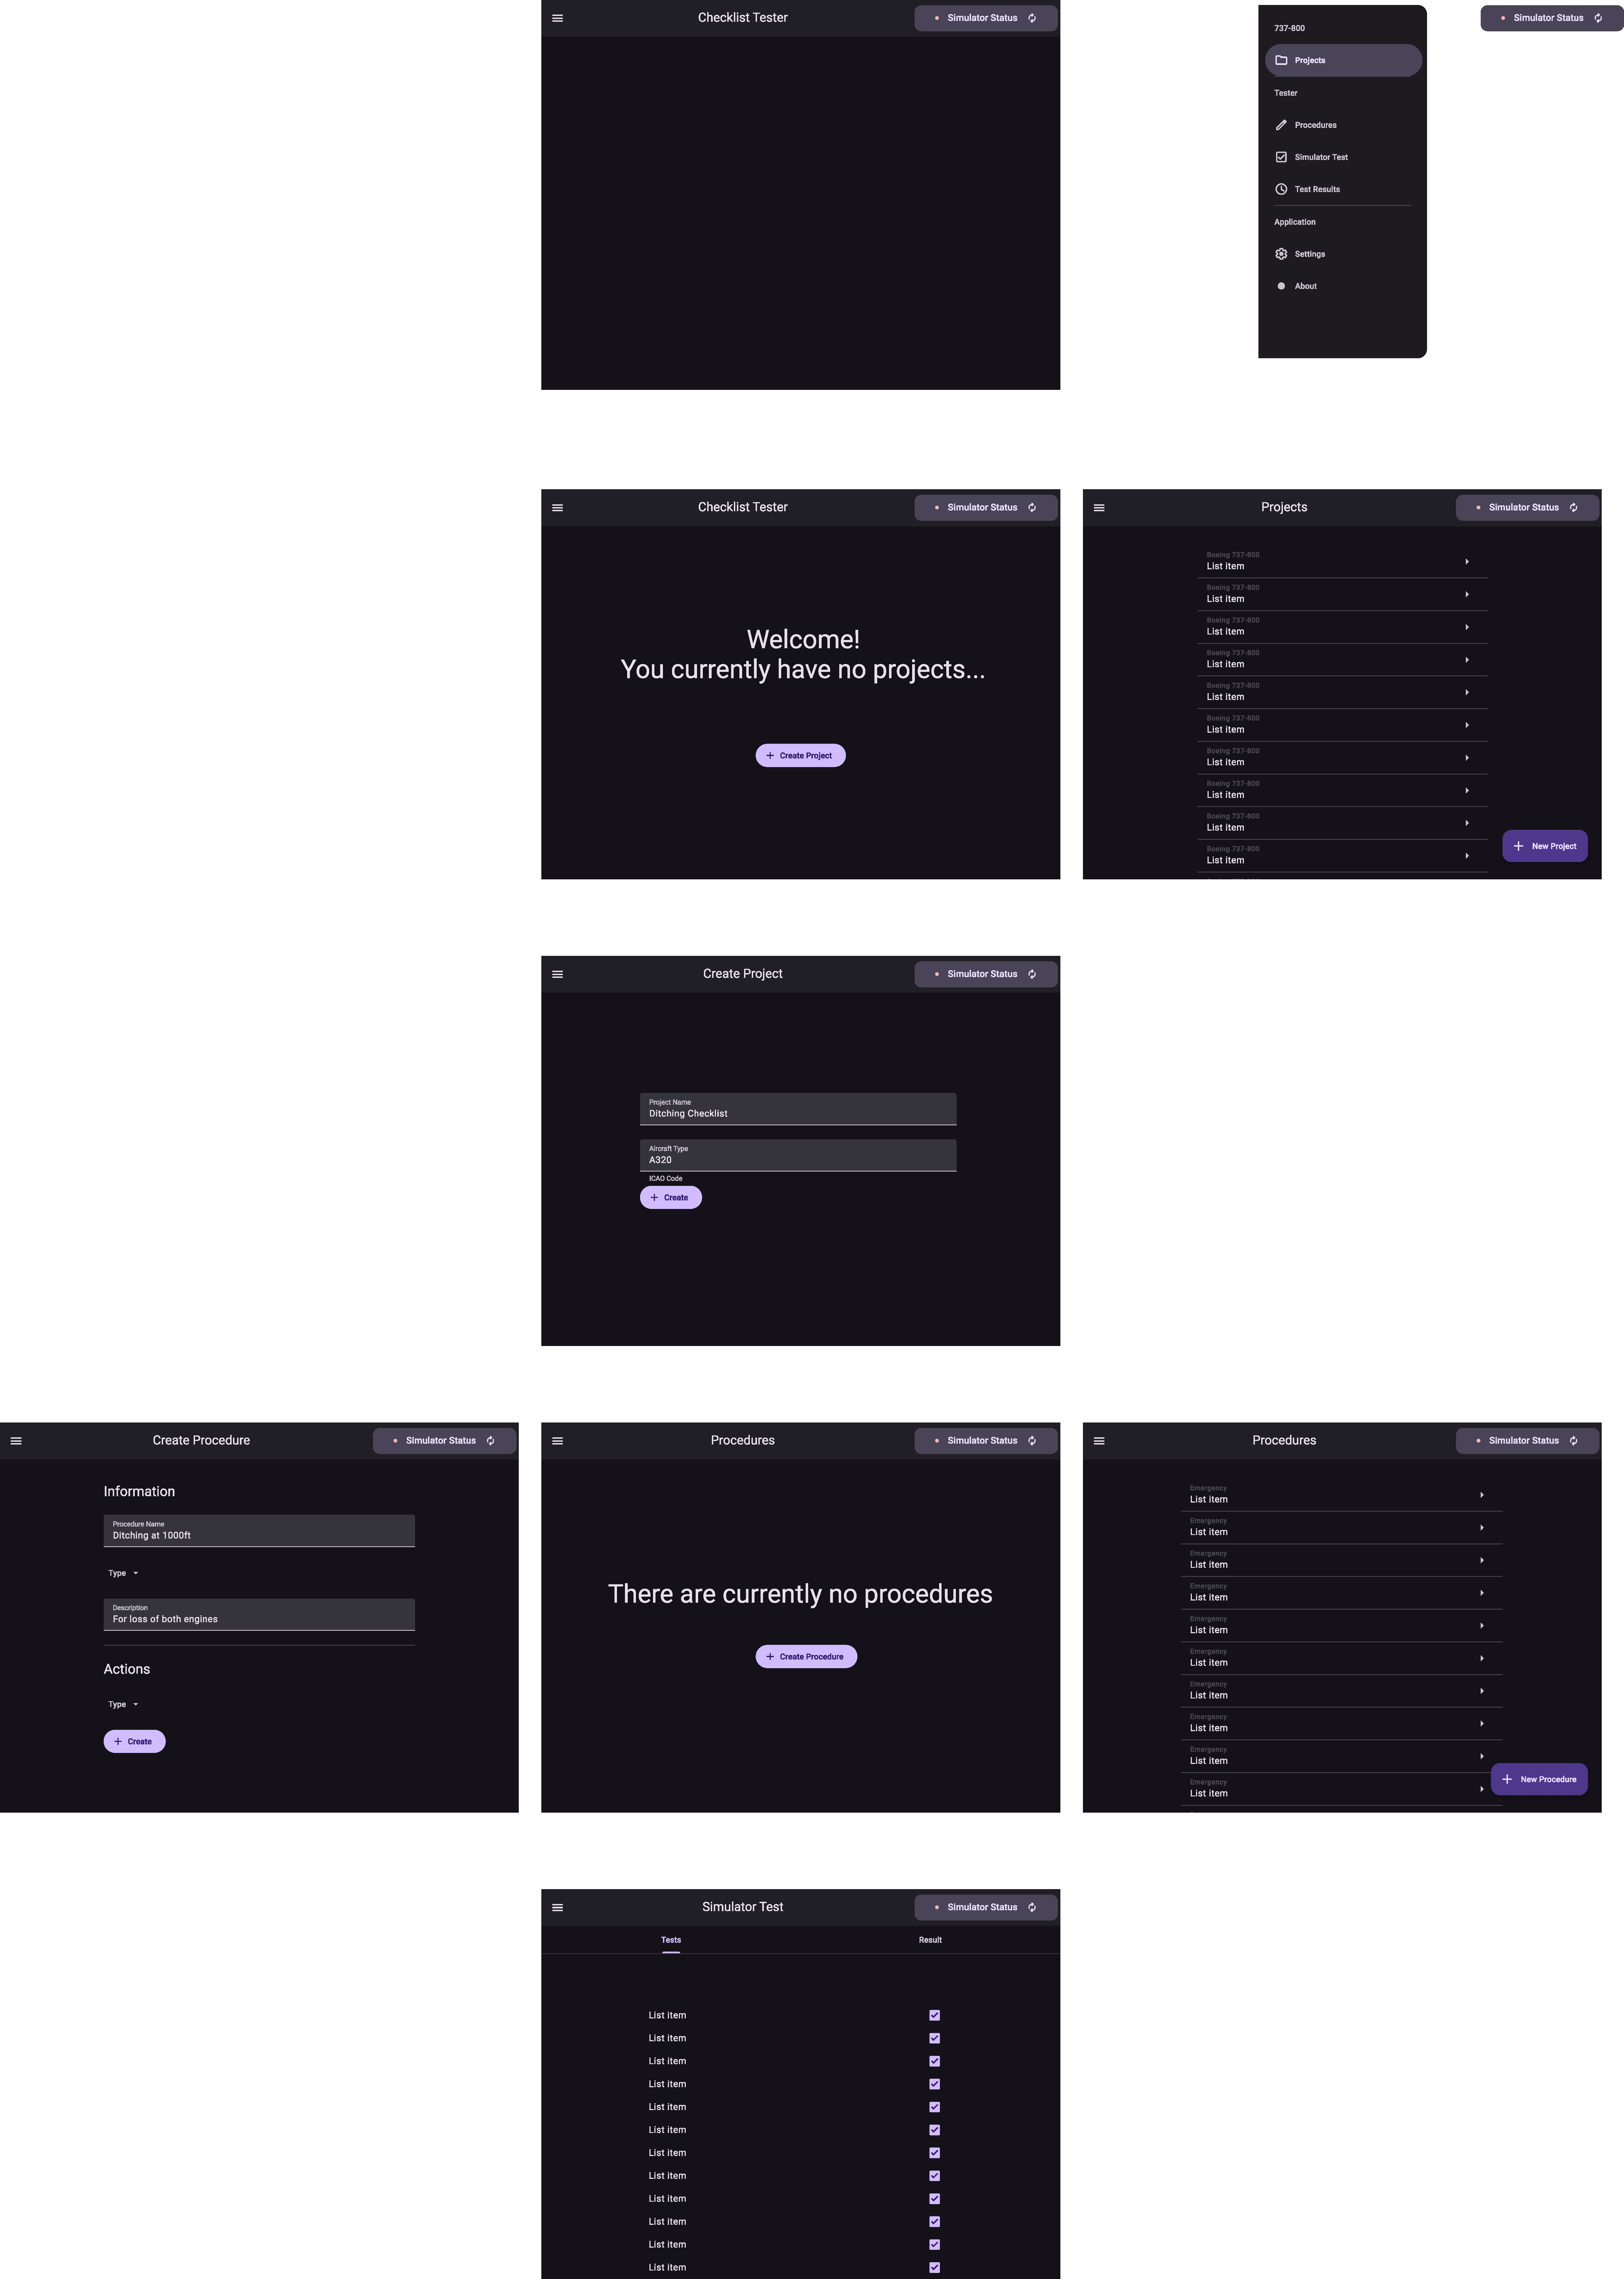
\includegraphics[width=\columnwidth]{images/figma-gui.pdf}
  \caption[GUI in Figma]{Design for the Checklist Connector GUI in Figma}
  \label{fig:figma-gui}
\end{figure}

\subsubsection{Limitations of Figma}
\begin{itemize}
  \item The Material 3 Components in Figma do not include features that are available in
    Jetpack Compose
  \item In this project, the \enquote{Simulator Test} at the bottom of \autoref{fig:figma-gui}
    does not include a leading icon~\cite{material:lists}, and therefore had to be a trailing
    checkbox
  \item This was overcome by adding comments in Figma as a reminder of how the actual implementation
    should be like
  \item Another limitation is that in \autoref{fig:figma-gui}, the title of the screen in the
    top app bar~\cite{material:top-app-bar} is not centred, and that is because the auto layout
    feature in Figma allows for equal spacing, rather than having each in a set position
\end{itemize}


\subsection{Compose Multiplatform}
\subsubsection{Setup}
\begin{itemize}
  \item Used the \textit{Kotlin Multiplatform Wizard} to create projects as it allows
    for runtime environments to be specified (in this case, Desktop and Server)
  \item Provides necessary build configurations in Gradle
  \item Planning what to implement important as Compose is designed to use modular
    components, otherwise a nested mess would occur as Compose is designed to have
    Composable functions passed in to a Composable function and therefore by design
    function nests will occur, and the code will be harder to read if not managed correctly.
    \autoref{list:compose-modular} shows example of using modular code
    from the Actions screen in project (with code omissions shown in comments)
  \item Used Voyager~\cite{voyager} to handle screens
  \item Used Koin~\cite{koin} for dependency injection, to be able to get data from the
    database and VDMJ
    \begin{itemize}
      \item Chose to use it because of Voyager integration with Koin~\cite{voyager:koin}
      \item Required as the application will be unresponsive when making requests
        to the database and/or VDMJ
      \item Used asynchronous coroutines to prevent the program from being blocked
    \end{itemize}
\end{itemize}

\begin{listing}
\inputminted[
  linenos,
  breaklines,
]{kotlin}{code/compose-modular.kt}
\caption[Compose Modular Example]{Example of modular code in Compose}
\label{list:compose-modular}
\end{listing}

\subsection{Storing Data}
\begin{itemize}
  \item SQLDelight was used to handle the database by allowing for typesafe Kotlin APIs when interacting with the database.
    Specifically chosen as it provides support for Compose Multiplatform~\cite{sqldelight}
  \item It only allows for queries to be written in SQL, which would allow for more complex SQL queries if needed
  \item SQLite was used for the Relational Database Management System (RDBMS) as it is an embedded database~\cite{sqlite:about},
    meaning that the database will run in the application, rather than running on a server,
    either remotely or through local containerization through something like Docker~\cite{docker:container},
    which could take more time and add complexity as it means implementing additional dependencies
  \item SQLite also has 100\%~\cite{sqlite:tests} test coverage which is necessary for ensuring that the database will
    not cause artefacts to the results
\end{itemize}

\subsubsection{Designing the Database}
\begin{itemize}
  \item The database could be thought as having 2 sections
    \begin{itemize}
      \item The user inputs to control the tester, i.e. the steps a procedure contains.
        The tables for these are \textit{Project}, \textit{Procedure}, and \textit{Action}
      \item The test results for a procedure which are in the \textit{Test}, and \textit{ActionResult} tables
    \end{itemize}
\end{itemize}

\begin{figure}[!htp]
  \centering
  \begin{tikzpicture}[
    auto,
    node distance = 1.5cm
  ]
    % PROCEDURE
    \node[entity] (procedure) {Procedure}
      [grow=up, sibling distance=2.25cm]
      child[grow=down] {node[attribute] {\textbf{id}}}
      child {node[attribute] {name}}
      child {node[attribute] {type}}
      child [grow=north west, level distance=2.15cm]{node[attribute] {description}}
      child [grow=right, level distance=3cm] {node[attribute] {createdUTC}}
      child [grow=left, level distance=3cm] {node[attribute] {modifiedUTC}};

    \node[relationship] (procProj) [above = of procedure] {Contains};

    % PROJECT
    \node[entity] (project) [right = of procProj] {Project}
      [grow=up, sibling distance=2cm]
      child {node[attribute] {name}}
      child {node[attribute] {\textbf{id}}}
      child {node[attribute] {aircraftType}}
      child[grow=right, level distance=3cm] {node[attribute] {createdUTC}}
      child[grow=south east, level distance=3cm] {node[attribute] {modifiedUTC}};

    \node[relationship] (procAct) [below left = of procedure] {Contains};

    % ACTION
    \node[entity] (action) [below left = of procAct] {Action}
      child[grow=up, level distance=2cm] {node[attribute] {step}}
      child[grow=right, level distance=2cm] {node[attribute] {\textbf{id}}}
      child[grow=north west, level distance=2cm] {node[attribute] {type}}
      child[grow=down, level distance=2cm] {node[attribute] {goal}};

    \node[relationship] (actionResult) [below right = of action] {Contains};

    % ACTION RESULT
    \node[entity] (result) [below right = of actionResult] {ActionResult}
      child[grow=up, level distance=2cm] {node[attribute] {\textbf{id}}}
      child[grow=left, level distance=3cm] {node[attribute] {startUTC}}
      child[grow=right, level distance=3cm] {node[attribute] {endUTC}}
      child[grow=south west, level distance=2cm] {node[attribute] {initState}}
      child[grow=south east, level distance=2cm] {node[attribute] {endState}};

    \node[relationship] (testAR) [above right = of result] {Contains};

    % TEST
    \node[relationship] (procTest) [below right = of procedure] {Contains};
 
    \node[entity] (test) [above right = of testAR] {Test}
      child[grow=left, level distance=2cm] {node[attribute] {\textbf{id}}}
      child[grow=north east, level distance=2cm] {node[attribute] {startUTC}}
      child[grow=south east, level distance=2cm] {node[attribute] {endUTC}};

    % RELATIONSHIP PATHS
    \path (procProj) edge node {\(N\)} (procedure)
      edge node {1} (project);

    \path (procTest) edge node {1} (procedure)
      edge node {\(N\)} (test);

    \path (procAct) edge node {1} (procedure)
      edge node {\(N\)} (action);

    \path (actionResult) edge node {1} (action)
      edge node {\(N\)} (result);

    \path (testAR) edge node {1} (test)
      edge node {\(N\)} (result);
  \end{tikzpicture}
  \caption[Connector ER Diagram]{Entity Relationship Diagram for the database in Checklist Connector}
  \label{fig:db-erd}
\end{figure}

\begin{itemize} 
  \item The design of the database had relationships in mind as the goal was to
    have a detailed tracking of statistics for each step in the procedure,
    hence in \autoref{fig:db-erd}
  \item A \textit{Procedure} can have multiple \textit{Tests}, where each \textit{Test}
    each contains the result of how each \textit{Action} in \textit{ActionResults}
  \item The choice of a \textit{Project} was to allow for the segregation of testing
    different aircrafts, as each aircraft has different cockpit layouts
    and different systems
\end{itemize}

\subsubsection{Implementing into Compose Multiplatform}
\begin{itemize}
  \item Compose Multiplatform has support for different runtime environments,
    however as this project was only being developed for Desktop, the JVM
    SQLite driver only had to be considered
  \item However, the functions for the database were written in the \textit{shared/commonMain}
    module as there may be a potential for adding Android and iOS support as it may be
    helpful run the tests on a tablet
  \item A database transaction had two modules
    \begin{itemize}
      \item A class handling SQLDelight API calls only; meaning no conversion of types, which are
        functions only accessible within module internally, which is located in\\
        \textit{io.anthonyberg.connector.shared.database}
      \item SDKs that can handle multiple tables, such as \textit{TestTransaction} which handles database calls
        when checklists are being tested in the application.
        And allows for converting types, such as \lstinline|Int| to \lstinline|Long|
    \end{itemize}
  \item The separation of these modules was to have in mind unit testing, as
    it will make it easier to debug if a problem is with SQLDelight transactions
    are handled, or if there is a conversion error occurring
\end{itemize}

\subsection{VDMJ Wrapper}
\begin{itemize}
  \item VDMJ is written in Java and it is free open source software that is accessible on
    GitHub
  \item This allows for VDMJ to be used as per the licence, GNU General Public License v3
    (GPLv3)~\cite{vdmj:license}~\cite{gpl3}. This means that as VDMJ is being used as a
    library, the code for this project has to be licensed with GPLv3 or any GPLv3 compatible
    licence~\cite{gpl3:library}
\end{itemize}

\subsubsection{Implementing VDMJ}
\begin{itemize}
  \item VDMJ has packages available on Maven Central making adding it as a dependency simple
  \item The package used was \lstinline|dk.au.ece.vdmj:vdmj| with version \lstinline|4.5.0|
  \item However, initially when implementing VDMJ, \lstinline|4.5.0-P| was used accidentally,
    and it led to debugging why imports were not working; and therefore the \lstinline|-P|
    versions are not suitable
  \item The initial method of implementation was using a Ktor server that would have run
    alongside the desktop application, where the server would handle Representational State Transfer (REST)
    API calls
  \item This was unnecessary as the \textit{interactive} mode of VDMJ was able to run on
    the desktop application itself. However, the Ktor was useful for debugging and testing as
    an API route was created to allow VDMJ commands to be executed through a URL

  \item To be able to get the outputs from VDMJ, a \lstinline|ConsolePrintWriter| new had to be
    created from the \lstinline|com.fujitsu.vdmj.messages| package; which handles writing to
    the console \textit{stdout}. This then gets used to replace the \lstinline|Console.out| and
    \lstinline|Console.err| in the \lstinline|com.fujitsu.vdmj.messages| package

  \item Parsing commands into VDMJ interface - was more difficult
    \footnote{The objects created here are provided by the \lstinline|java.io| package.}
  \begin{itemize}
    \item Created a \lstinline|PipedInputStream| object, that gets connected to a \lstinline|PipedOutputStream|
      object by passing the latter object in as a parameter. The \lstinline|PipedOutputStream| is then used
      to pass inputs into \lstinline|PipedInputStream|
    \item To be able to write to this stream, a \lstinline|BufferedWriter| is created by passing the \lstinline|PipedOutputStream|
      with a bridge \lstinline|OutputStreamWriter| that encodes characters into bytes
    \item For VDMJ to be able to read the input stream, a separate object had to be created, \lstinline|BufferedReader|,
      where the \lstinline|PipedInputStream| gets parsed through a bridge, \lstinline|InputStreamReader| that converts
      bytes to characters
      % TODO create a diagram of this (better than having code)
      % BufferedWriter -> encode to byte -> Stream -> decode to char -> VDMJ
  \end{itemize}
\end{itemize}

\begin{figure}[!htp]
  \begin{tikzpicture}[node distance=2cm, align=center]
    \node (write) [box] {Run VDM command};
    \node (buffWrite) [box, below of=write] {BufferedWriter};
    \node (outputStream) [box, below of=buffWrite] {Encode to byte};
    \node (pOutputStream) [box, below of=outputStream] {PipedOutputStream};
    \node (pInputStream) [box, right of=pOutputStream, xshift=3cm] {PipedInputStream};
    \node (inputStream) [box, above of=pInputStream] {Decode to charset};
    \node (buffRead) [box, above of=inputStream] {BufferedReader};
    \node (vdmj) [box, above of=buffRead] {Read by VDMJ};

    \draw[->, arrow] (write) -- (buffWrite);
    \draw[->, arrow] (buffWrite) -- (outputStream);
    \draw[->, arrow] (outputStream) -- (pOutputStream);
    \draw[<->, arrow] (pOutputStream) -- (pInputStream);
    \draw[->, arrow] (pInputStream) -- (inputStream);
    \draw[->, arrow] (inputStream) -- (buffRead);
    \draw[->, arrow] (buffRead) -- (vdmj);
  \end{tikzpicture}
  \centering
  \caption[VDMJ IO Stream]{Flowchart of VDMJ Input/Output Stream handling}
  \label{list:vdmj-io}
\end{figure}


\subsubsection{Handling VDMJ Outputs}
\begin{itemize}
  \item VDMJ outputs are handled using string manipulation
  \item Created into objects that are replicas of types in VDM-SL
  \item The string manipulation allows specifying where the outputs
    of the object go
\end{itemize}


% Talk about how XPC was used here, not how it was implemented
\subsection{Connecting to the Flight Simulator}
\begin{itemize}
  \item Implemented XPC into the flight simulator
  \item Allowed being able to
  \begin{itemize}
    \item Read data from the simulator
    \item Override dataref variables in the simulator
    \item Execute other commands that can manipulate certain switches
      where otherwise unable to by changing the value of the dataref
  \end{itemize}
  \item Made sure to check that the simulator is connected before running
    the test to avoid exceptions being thrown
  \item Logic behind doing an action is to fetch the action's initial state
    from the dataref variable name, run the action, then get the final state
    of the dataref
  \item There is an artificial delay added before running the action to
    try and simulate a delay of the crew's lag between reading the step of the
    checklist and doing the action
  \item Because of this, XPC had to be run asynchronously to prevent the
    GUI from hanging as a function is waiting to complete - prevents misleading
    user that the application has crashed, and it looks better 
\end{itemize}


\subsection{Testing}
\begin{itemize}
  \item Testing can be run with Gradle when it comes to running unit tests
  \item Decided to use JUnit 5 as it provides additional tools such as
    statistics, integration with IntelliJ to view code coverage,
    or being run in continuous integration tests
  \item The testable components in this project is mostly backend modules as
    the GUI made in Compose is not the focus of the project, and it would
    require a lot of extra time
  \item Unit tests have been made for the database and Koin
  \item Koin comes with tests that can be automatically be generated
  \item Ethos when testing was to try and find exploits, act as a
    user who may mishandle inputs, and stress testing functions
    by passing parameter with hundreds of objects
\end{itemize}

\subsubsection{Testing for Resource Usage}
\begin{itemize}
  \item The application was tested using the \textit{Profiler} tool on
    IntelliJ IDEA 2024 (Ultimate Edition) to find potential
    memory leaks
  \item One problem found was the initial VDMJ wrapper which would use the execute
    command instead of the interpreter, which would require reinitializing
    the entirety of VDMJ, which resulted in a slight memory leak and a
    massive write usage
\end{itemize}



%%%%% Simulator Connector Plugin %%%%%
\section{Simulator Connector Plugin}
% Talk about creating your own (originally happened) vs using something else that was developed
% Maybe talk about original plan? i.e. <project root>/plugin


\subsection{Creating Maven Package}
% Gradle
% Testing
% GitHub CI
\begin{itemize}
  \item XPC package is not published on a public Maven repository
  \item There has been a pull request that was merged to the \textit{develop} branch
    that provides Maven POMs~\cite{xpc:pom}. However, the maintainer for the
    project, at the time, did not have enough time to figure out the process of
    publishing the package to a Maven repository~\cite{xpc:pom-time}
  \item Therefore, had to find an alternative way to implement
  \item Jitpack~\cite{jitpack}
  \begin{itemize}
    \item In theory, simple to publish a repository, all that is required is a GitHub
      repository and searching if one has already been created on JitPack or build and publish
      a specific version
    \item However, due to the structure of the XPC repository, JitPack could not locate the
      build tools (Apache Maven in this case) as JitPack only searches on the root directory
      for the compatible build tools
  \end{itemize}
  \item Gradle gitRepository~\cite{gradle:gitRepository}
  \begin{itemize}
    \item There was not a lot of documentation
    \item Ambiguous on how to define directory for where the Java library is located in the Git repository
    \item However, as XPC was only built with Maven, Gradle was not able to add the dependency as \lstinline|gitRepository()|
      only works with Gradle builds~\cite{gradle:gitRepoGradleOnly}
  \end{itemize}
\item Resorted to using a compiled Jar file and adding the dependency to Gradle
\item Not happy about that because it means maintaining it will be more difficult as
  it is not as simple as just changing the version number
\item Later, resorted to adding Gradle build files to XPC
\item Used automatic conversion from Maven to Gradle using \lstinline|gradle init| command~\cite{gradle:migratePOM}
\item Had to add local dependencies due to how Gradle works differently
\item Had to fix previous structure of Maven POM as the grouping as not good
\end{itemize}

\subsubsection{Continuous Deployment of the Maven Package}
\begin{itemize}
  \item Used GitHub's template for Gradle package publishing
  \item Required some setup in Gradle build files
\end{itemize}

\subsection{Submitting a Pull Request}
% What I did:
% - gitignore
% - changing url for repo
% - testing everything still worked
\begin{itemize}
  \item Adding the Gradle build tools can be seen as being helpful
    for others, as it would allow for the XPC library to be added
    as a dependency, especially if the NASA Ames Research Center Diagnostics and Prognostics Group
    were to add it to the GitHub repository, it would mean that it would be easier for
    people to access Maven Packages for XPC
  \item Therefore, to help improve the experience for other people who would want
    to develop with the XPC Java library, it would be logical to submit a
    pull request
  \item But it did mean making sure that the contribution would be perfect and not contain problems % TODO Improve wording
\end{itemize}

\subsubsection{Testing}
\begin{itemize}
  \item The XPC Java library includes a JUnit 4 test, however, implementing this
    with Gradle proved useless, as it was not able to get the results from the
    tests, which would be bad for not being able to catch problems with new builds
  \item Therefore, the tests were updated to JUnit 5, where most of the changes were
    adding asserts for throws~\cite{junit:migrate}
    \footnote{The commit including the changes to the tests can be viewed here:
    \url{https://github.com/smyalygames/XPlaneConnect/commit/e7b8d1e811999b4f8d7230f60ba94368e14f1148}}
\end{itemize}

\subsubsection{GitHub}
\begin{itemize}
  \item Made sure to add generated build files to .gitignore
  \item Changed the URL of the repository in Gradle to NASA's repository so that
    the Maven package can be published correctly on the GitHub repository
  \item From the beginning anyways, made sure to have insightful commit messages
  \item Submitted the pull request stating the changes made\footnote{\url{https://github.com/nasa/XPlaneConnect/pull/313}}
\end{itemize}



%%%%% SCENARIOS %%%%%
\section{Scenarios}
\begin{itemize}
  \item Use a Quick Reference Handbook (QRH) to find potential list of checklists to test
  % TODO find these accident reports
  \item Look at previous accident reports that had an incident related to checklists
    and test it with my tool to see if it will pick it up
  \item These previous accident reports can be good metrics to know what statistics to
    look out for
\end{itemize}


%%%%% DECISIONS %%%%%
\section{Decisions}
\end{document}
